\documentclass[12pt,a4paper]{article}
\usepackage[utf8]{inputenc}
\usepackage[portuguese]{babel}
\usepackage{graphicx, hyperref}

\author{Grupo 154 \and João Daniel Silva 86416 \& Francisco Sousa 86416}
\title{Relatório 2º Projecto de ASA}
\begin{document}
\maketitle

\section{Introdução}
No âmbito do segundo projeto da cadeira de Análise e Síntese e Algoritmos, foi-nos proposto um problema de segmentação de imagens,
no contexto da análise de imagens obtidas de cameras de carros autómatos.

Considerando que uma imagem é um conjunto de pixeis, pretende-se que cada um seja classificado como sendo de primeiro plano ou de
cenário. No enunciado foi definido que o algoritmo a utilizar consistiria num processo de minimizar uma soma de peso, ou seja, o
problema pode ser representado como um problema de fluxos.

Cada vértice tem um peso de primeiro plano \textit{lp}, cenário \textit{cp} e de
vizinhança \textit{fv}. Todos estes pesos contribuem para a soma de peso total. Cada vértice tem 4 vizinhos, o de cima, o de baixo, o
da esquerda e o da direita. O peso total de uma segmentação é calculada com a seguinte fórmula:

$$\sum_{p \in L} \textit{lp} + \sum_{p \in C} \textit{cp} + \sum_{v \in V} \textit{fv} $$

Para modelar este problema recorremos à teoria de grafos para representar \textbf{fluxos}. É criado um grafo dirigido e pesado, em que cada
vértice corresponde a um pixel, cada arco entre dois vértices tem uma capacidade e pode receber um fluxo. Ao conjunto de vértices
que representam os pixeis são adicionados dois que representam a \textbf{source} e a \textbf{sink}.

A source conecta-se a todos os pixeis e cada
aresta tem a capacidade correspondente ao peso de primeiro plano de cada vértice; analogamente, todos os vértices conectam-se
à sink com a capacidade correspondente ao peso de cenário; cada aresta entre pixeis vizinhos tem a capacidade da vizinhança
definida no input.

Implementámos a nossa solução na linguagem de programação C++ para facilitar a implementação de estruturas de dados. O
algoritmo escolhido para a resolução do problema de fluxos foi o \textbf{Algoritmo de Edmonds-Karp}, pois tem uma implementação relativamente
simples em relação a outros, como o \textbf{Algoritmo de Dinic}.

\section{Descrição da Solução}
\subsection{Estruturas}
Cada vértice é representado por uma \textbf{struct vértice} que armazena a capacidade da rede residual das ligações aos seus
4 vizinhos (\textit{north}, \textit{south}, \textit{east}, \textit{west}). Como a source e a sink se podem ligar a todos os vértices,
optámos por representar
em cada \textbf{struct vértice} também a capacidade da rede residual da ligação de cada vérice a estes dois, evitando criar
uma estrutura separada que armazenasse as V-ligações que a source e a sink têm.

Como apenas armazenamos a capacidade da aresta, para sabermos a que vértice a aresta aponta definimos as funções
\textbf{relatdPos} e \textbf{getVertixInDir} que devolvem, respetivamente, a direção entre dois vértices e o vértice apontado
dada uma direção. Estas funções serão chamadas quando for necessário percorrer os vértices adjacentes de um vértice.

\subsection{Algoritmo}
Ao ler o input, é criado o grafo de $NxM$ vértices e de seguida a rede residual de cada aresta e das suas inversas é atualizada.

Para otimizar o tempo de execução, antes de aplicar o \textbf{Edmonds-Karp}, atualizamos para cada vértice a rede residual entre a
\textit{source-vértice-sink} para o mínimo dos flows que é possível passar nas ligações \textit{s-vértice} e \textit{vértice-sink}.
Assim, reduzimos número de arcos que a \textbf{BFS} irá percorrer para procurar \textit{augmenting paths} durante o \textbf{Edmonds-Karp}.

Para facilitar a implementação da \textbf{BFS}, usamos a queue do \textbf{std::queue}; como não armazenamos os vértices adjacentes à source,
temos de percorrer todos os vértices e verificar se ainda é possível receber flow da source, e posteriormente adicioná-los
à queue.

De seguida, corremos a \textbf{BFS} de forma convencional, atualizando o \textbf{array pi}, que representa o predecessor
de cada vértice, que terá a informação do caminho mais curto. Após ser verificado quanto flow pode ser enviado, as ligações
são atualizadas. Este processo é repetido enquanto houver um \textit{augmenting path}. Ao finalizar o algoritmo, é devolvido o \textit{max-flow} do fluxo.

O teorema \textit{max-flow} \textit{min-cut} afirma que o valor máximo do fluxo desde a source até à sink é igual ao peso das arestas no
\textit{min-cut}. Com isto em mente, percorremos uma \textbf{DFS} desde a source e verificamos quais vértices são possíveis de descobrir.
Esses serão os vértices que farão parte do cenário e os restantes serão os de primeiro plano.

\section{Análise}
\subsection{Teórica}
O algoritmo \textbf{Edmonds-Karp} tem complexidade $O(V{E}^2)$. A cada iteração, o tamanho do caminho mais curto desde a source até
aos outros vértices varia de forma monótona crescente, pois os mais curtos são sucessivamente esgotados, tendo cada
caminho no máximo O(E) arestas. O número máximo de iterações é V*E, pois há O(E) pares de vértices que para cada dois
vértices u e v podem ficar saturados O(V) vezes.

Na separação dos pixeis em dois grupos de vértices na deteção do \textit{min-cut} a \textbf{DFS} demora $O(V+E)$, no entanto é majorada
pelo \textbf{Edmonds-Karp}.

Assim, podemos concluir que a complexidade final do algoritmo é $O(V{E}^2)$.

\subsection{Experimental}
Para esta análise utilizámos o gerador de inputs disponibilizados pelos docentes.
Apoiados pelo gráfico \ref{g1}, podemos verificar que a execução do algoritmo é polinomial de grau 2, em relação ao número de vértices.


A diferença em relação à análise teórica pode-se explicar pelo facto de que, para os inputs gerados, a procura de caminhos mais curtos
na \textbf{BFS} do \textbf{Edmonds-Karp} não precisa de percorrer muitas arestas, se as ligações que saiem da source ficam saturadas rapidamente.
Esta saturação também é acelerada pelo processo de saturação das ligações \textit{s-vértice} e \textit{vértice-sink} explicado acima, antes da execução do \textbf{Edmonds-Karp}.

O pequeno desvio do gráfico é explicado pelos processos a correr em paralelo no computador, que interferem na execução.

\begin{figure}[h]
			\centering
			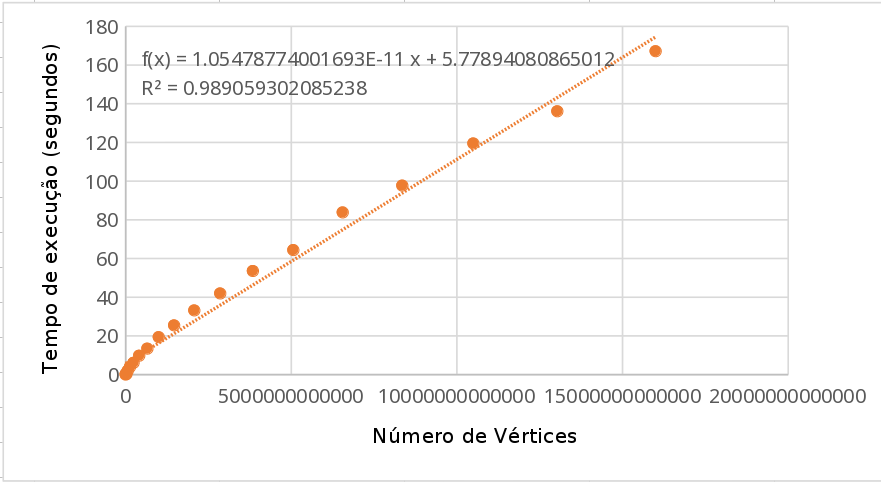
\includegraphics[width=0.5\textwidth]{graph}
			\caption{Variação do número de vértices {V}² em função do tempo de execução do programa}
			\label{g1}
\end{figure}

\section{Referências}
\begin{itemize}
	\item \href{https://www.geeksforgeeks.org/ford-fulkerson-algorithm-for-maximum-flow-problem/}{https://www.geeksforgeeks.org/ford-fulkerson-algorithm-for...}
	\item \href{https://brilliant.org/wiki/edmonds-karp-algorithm/}{https://brilliant.org/wiki/edmonds-karp-algorithm/}
\end{itemize}
\end{document}
